\documentclass{beamer}
\usetheme{Goettingen}
\usepackage{hyperref, graphicx}
\begin{document}
%\nocite{voss2007essentials}
\title{Chapter 8: Maps and related tasks}  
\author{Harm Dermois \and Joris Stork}
\date{\today} 

\frame{\titlepage} 
\frame{\tableofcontents} 

\section{Robots and maps} 

\frame{\frametitle{Maps for robots}
\begin{columns}[c]
\column{5cm}
Human maps:
\begin{itemize}
    \item Often unavailable; 
    \item Often incomplete: %blueprint image
    \begin{itemize}
        \item human relevant data; %obstacles within a building like chairs and tables.
        \item robot relevant data;
    \end{itemize} 
\end{itemize}
\column{5cm}
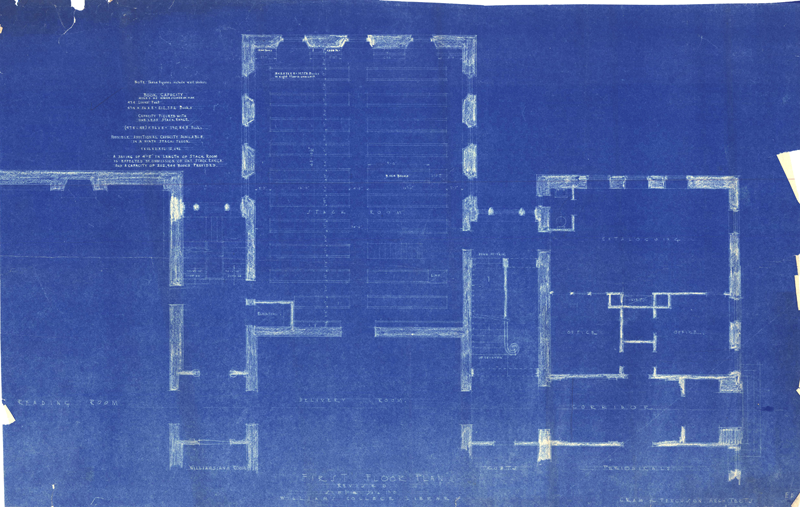
\includegraphics[width=5cm]{blueprint}
\end{columns}
}

\frame{\frametitle{Maps for robots}
\begin{columns}[c]
\column{5cm}
Human maps:
\begin{itemize}
    \item Often unavailable; 
    \item Often incomplete: %blueprint image
    \begin{itemize}
        \item human relevant data; %obstacles within a building like chairs and tables.
        \item robot relevant data;
    \end{itemize} 
    \item Wrong level(s) of abstraction: human oriented; %pizzas on googlemaps 
\end{itemize}
\column{5cm}
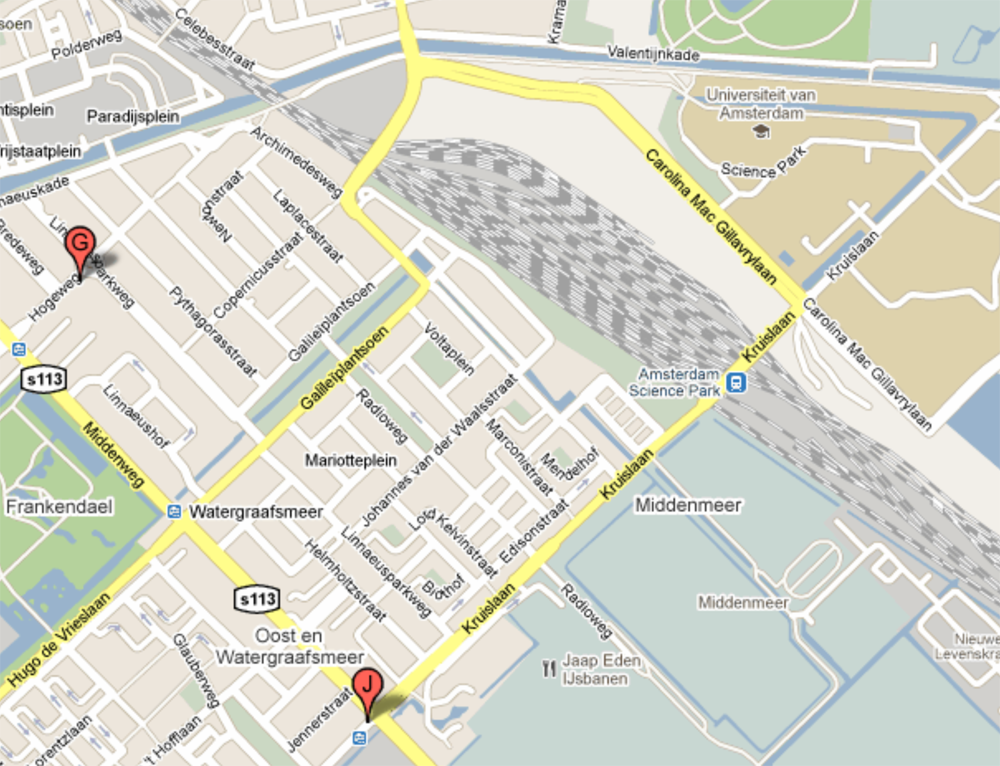
\includegraphics[width=5cm]{google_pizzas}
\end{columns}
}

\frame{\frametitle{Maps by robots}
\begin{itemize}
    \item
        Building a robot friendly map is very difficult and tedious.
    \item
        Robots are good candidates to build maps with and for their own sensory
        suite;
\end{itemize}
Conclusion: Design robots to autonomously construct, update and validate
maps destined for robot use.
}

\frame{\frametitle{Map paradigms: metric vs. topological}
\begin{columns}[c]
\column{5cm}
\begin{itemize}
    \item Metric %something from wikipedia
        \begin{itemize}
        \item Sensorial
        \item Geometric
        \end{itemize}            
\end{itemize}
\column{5cm}
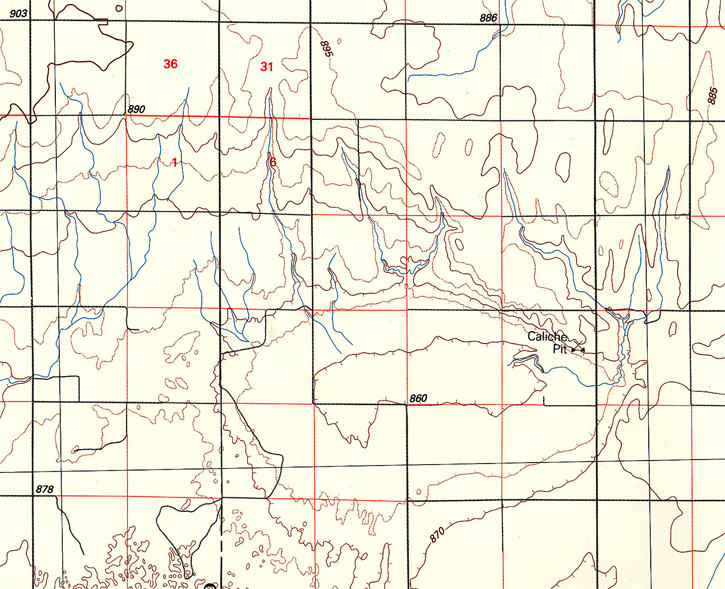
\includegraphics[width=5cm]{metric}
\end{columns}
}

\frame{\frametitle{Map paradigms: metric vs. topological}
\begin{columns}[c]
\column{5cm}
\begin{itemize}
    \item Metric %something from wikipedia
        \begin{itemize}
        \item Sensorial
        \item Geometric
        \end{itemize}            
    \item Topological %put a picture of the london underground
        \begin{itemize}
        \item Local relational
        \item Topological
        \item Semantic
        \end{itemize}            
\end{itemize}
\column{5cm}
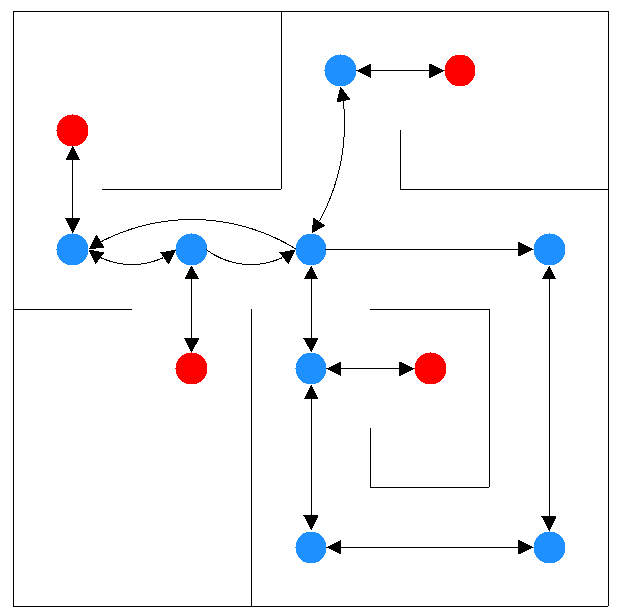
\includegraphics[width=5cm]{topological}
\end{columns}
}

\frame{\frametitle{Direction of map hierarchy}
\begin{itemize}
    \item Giralt et al.: metric to topological. 
    \item Kuipers and Levitt: topological to metric. Low level topological
    landmarks as starting point.
\end{itemize}
}

\frame{\frametitle{Types of data}
\begin{itemize}
    \item (Derived) spacial occupancy; 
    \item (Direct) sensor measurements in relation to position. e.g. olfaction.
\end{itemize}
}

\section{Sensorial maps}

\frame{\frametitle{Sensorial maps}
\begin{itemize}
    \item Represent sensor measurements against odometry; 
    \item Collection of measurements: $[I_i(x_i,y_i,\theta_i)]$
\end{itemize}
}

\subsection{Image based mapping}
\frame{\frametitle{Image based mapping}
The challenge: 
\begin{itemize}
    \item how to sample the set of possible measurements,
    $\lbrace I_i\rbrace$;
    \item how to turn the samples into a continuous $I$.
\end{itemize}
}

\frame{\frametitle{Li: street panoramas}
Li et al.: robots builds graph representing street network:
\begin{itemize}
    \item edges = streets;
    \item nodes = intersections;
\end{itemize}
Robot collects by:
\begin{itemize}
    \item moving in a closed loop, always turning left;
    \item recording panoramas of left and right sides of streets;
    \item concluding a loop by identifying previously recorded street side;
\end{itemize}
}

\frame{\frametitle{Bourque: robot sightseeing}
Bourque et al.: robots builds graph nodes corresponding to panorama shots, in a
less constrained environment, by:
\begin{itemize}
    \item choosing sample (panorama) points based on models of human attention;
    \item using ``alpha backtracking'' to make trade-off between distance to
    next sample point and optimality of next sample point;
\end{itemize}
}

\subsection{Spacial occupancy representations}

\frame{\frametitle{Spacial occupancy representations}
\begin{itemize}
    \item Grid of pixels
\end{itemize}
}

\frame{\frametitle{Volumes}
\begin{columns}
\column{5cm}
\begin{itemize}
    \item Grid of pixels
    \item Volume of voxels
\end{itemize}
\column{5cm}
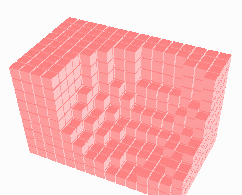
\includegraphics[width=5cm]{voxels}
\end{columns}
}

\frame{\frametitle{Data represented}
\begin{itemize}
    \item Fill pixels / voxels with degree of occupancy data.
    \item More refined: fill pixels / voxels with probability of occupancy data.
\end{itemize}
}

\frame{\frametitle{Probability}
\begin{itemize}
    \item Example of a laser: probability of an actual distance $z$ for a given laser
    reading $r$ computed using Bayes' theorem:
    \begin{eqnarray}
        P(z\lvert r) = \frac{P(z) P(r \lvert z)}{P(r)}
        \nonumber
    \end{eqnarray}
    
    \pause
    \item Generalised:
    \begin{eqnarray}
        P(W\lvert R) = \frac{P(W) P(R \lvert W)}{P(R)}
        \nonumber
    \end{eqnarray}
    with $P(R_i)=\sum_j P(R_i \lvert W_j) P (W_j)$
\end{itemize}
}

\subsection{Geometric maps}
\frame{\frametitle{Geometric maps}
}

\frame{\frametitle{Blah}
\begin{columns}[c]
\column{5cm}
\column{5cm}
% 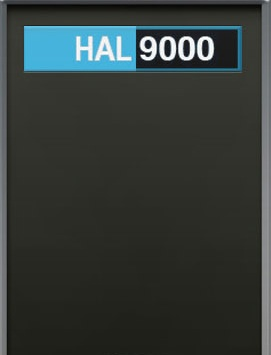
\includegraphics[width=5cm]{halsub1}
\end{columns}
}

\section{Topological Maps}

\begin{frame}{Topolgical Maps}
 \textbf{Topological maps}: describes the environment as a graph that connects specific locations in the world and represents them as nodes(vertices).
 \begin{itemize}
 	\item Because metric representations cost too much memory to maintain in the long run.
 	\item Easy to understand for humans.
 \end{itemize}
 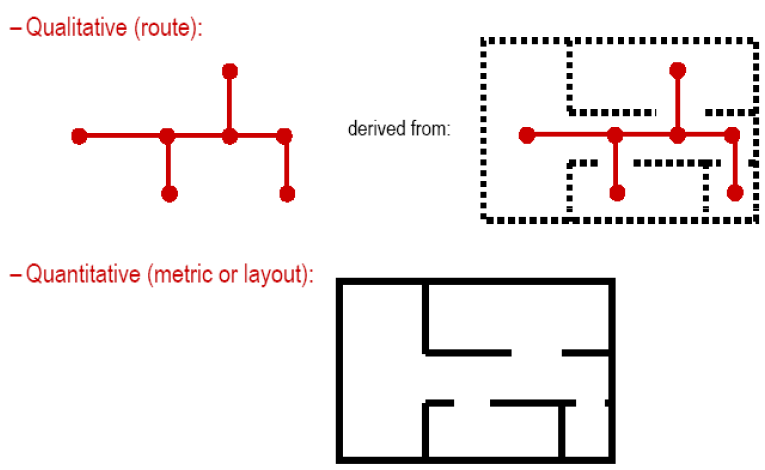
\includegraphics[scale = .4]{topovsmetric.png}
\end{frame}

\begin{frame}{The Graph}
	\textbf{Landmarks and Edges}
	\begin{itemize}
		\item The nodes on the graphs are landmarks or features of the environment. 
		\item The edges are paths between the landmarks.
		\item Landmarks need to be unique to good landmarks.
		\item Landmarks can be artificial or natural.(junctions, signs)
	 	\item The graph can be extended by enumerating the edges incident to the node entered. Edge you traveled along is 0 and enumerate clockwise. This enumeration is local cause it depends on the edge the robot moved over.
	\end{itemize}	
\end{frame}

\begin{frame}{Marker Based Exploration}
	\textbf{Marker Based Exploration}: can be used when no prior information about the environment available and there aren't enough unique landmarks.
 \begin{itemize} 
 	\item The robot needs to have something to mark where it has already been.(spray paint, bread crumbs)
 	\item Here we choose marks which it can pick up, drop and recognize.
 	\item Using marks to explore has a $O(N^{3})$. They say.
 \end{itemize} 
\end{frame} 

\begin{frame}{Marker Based Exploration}	
	\begin{itemize}
		\item Iteratively builds up the known graph by traveling along the incident edges of a node.
		\item $v_{i}$ is the node where the robot is currently at. $v_{j}$ is the node where the robot is moving to. $E_{i,j}$ is the edge between the two nodes.
		\item In the transition function r stands is the edge number from the perspective of the last edge it came from.
		\item Transition function need to follow these properties. If $(v_{i},E_{i,j},r) = v_{j} $ and $(v_{j},E_{i,j},s) = v_{k} $, then $v_{j},E_{i,j},-s) = v_{i}$\\ Moves are invertible and can be retraced.
		\item $t \neq -s$ then $v_{j},E_{i,j},-s) = v_{i}$ and  $(v_{j},E_{i,k},s) = v_{j}$ are not valid. To avoid redundant and degenerate paths.
		\item Subgraph S for explored edges and Nodes. U is the for unexplored sub graph.
	\end{itemize}
\end{frame}

\begin{frame}{Marker Based Exploration}
	\textbf{Edge Ordering}: A correct graph.
	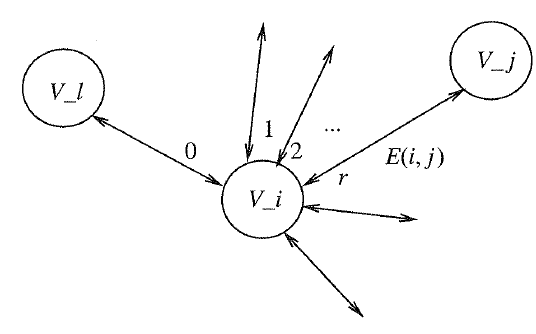
\includegraphics[scale= 0.6]{edgeordering.png}
\end{frame}

\begin{frame}{Marker Based Exploration}
	\textbf{Operations of the robot}
	\begin{itemize}
		\item Move along edge r.		
		\item Each marker can be in 3 different states[pickup,putdown,null]
		\item At each vertex the robot can see two things [present, not-present]
		\item Robot can determine the relative positions of the edges by enumerating the edges. So if a Robot enters the same vertex from a different edge gives two different orderings. The robot needs to make a global ordering.
	\end{itemize}
\end{frame}

\begin{frame}
	\textbf{Marker Based Exploration Example}
	\begin{itemize}
		\item First validate all explored nodes. So all nodes in graph S. Make sure there aren't any doubles by looking for markers.
		\item	Explore new nodes. If there is no marker found at a certain node v add it the subgraph S and add the edge which was taken aswell.
		\item Enumerate all edges incident to the new node and add them to U. 
		\item Do this till subgraph U is empty.
	\end{itemize}
	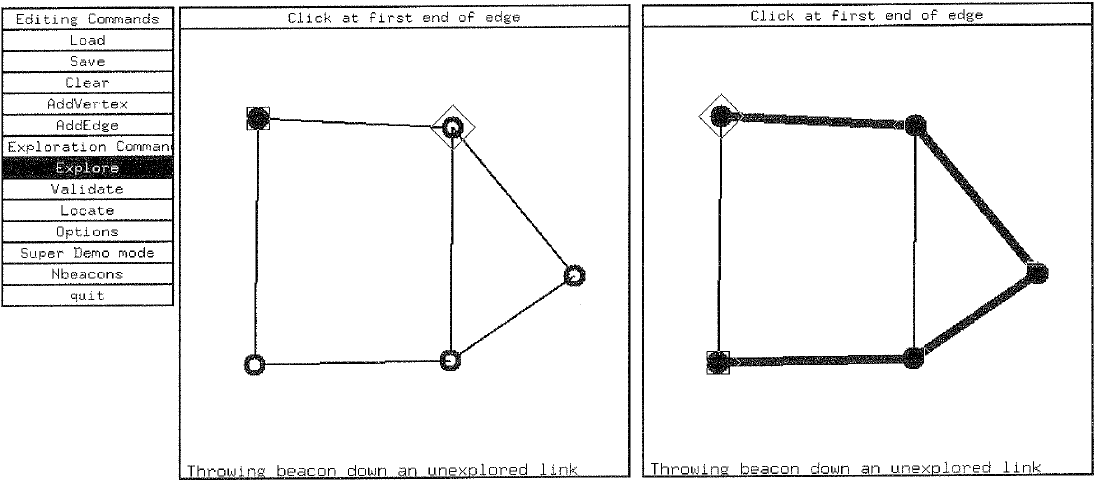
\includegraphics[scale =0.3]{voorbeeld.png}
\end{frame}

\section{Multiple Robots}
\begin{frame}{Multiple Robots}
	\textbf{Why would you use multiple Robots}
	\begin{itemize}
		\item \textbf{Improved Robustness}: A multirobot can, in principle, keep functioning even if one indiviudual robots dail completely. 
		\item \textbf{Improved effiency}: It is possible for a group of robots to accomplish a search or exploration task faster than an equivalent single robot.
		\item \textbf{Alternative Algorithms}: For some tasks, the availability of multiple robots allows feadible or guaranteed algorithms to be implemented when no such algorithm is available for a single robot system. 
	\end{itemize} 
\end{frame}

\begin{frame}{Multiple Robots in Practice}
	\textbf{Problems}
	\begin{itemize}
		\item \textbf{Where are the other robots?}: Rendezvous with other robots
		\item \textbf{Partitioning}: Finding a good way to distribute the work amongst the robots.
		\item \textbf{Multi-robot planning}: Prevent the trajectories of the robots to collide. 
		\item \textbf{Merging the data from the indivual team members}: Need to be close proximity and Sensor fusion problems.
	\end{itemize}	
\end{frame}

\begin{frame}{Rendezvous}
	\textbf{Rendezvous}: Is a having two or more robots meet at an appointed place and time. 
	\begin{itemize}
		\item A rendezvous is needed for robots that can only communicate in close proximities, but may also be needed to exchange objects between robots.
		\item When Multiple robots try to complete a task collaboratavely without prior knowledge. They need to to exchange information while they are still working at the task at hand.  
		\item	If they dont meet they cannot benefit from what others have already learned. 
	\end{itemize}
\end{frame}

\begin{frame}{Too many rendezvous}
	\textbf{Problems}:Robots mustn't devote too much energy to rendezvous to stay efficient.
		\begin{itemize}			
			\item The extent to which the two robots agree on their perceptions of the environment.
			\item The degree of synchornization of the robots can attain expressed as the likelihood that an appointed rendezvous at a common location will fail owning to a failure to arrive at the same time
			\item The extent of the commonality between the region of space the robots have explored.(Can't share if the parts are completely diffent)
		\end{itemize}
\end{frame}

\begin{frame}{Map Fusion}
	\textbf{Map Fusion}: is needed to make the collaborative efforts worthwhile when the problem needs a long term map.
	\begin{itemize}
		\item Complexity of the map-merging depends on the, Odemetry error, the fidelity of the sensing and the richness of the evironment.
		\item Fusing maps is mostly done by cross correlation. This depends on the fact that the individual maps overlap "sufficiently`.
		\item Done by rotation and translating the given maps to minimize the difference between them.
	\end{itemize}	
\end{frame}

\begin{frame}{Exploration with Multiple robots}
	\textbf{The basic idea of the algorithm}: Given Robots are only allowed to communicate when they are in the same node.
	\begin{itemize}
		\item Split all the work between all the robots and have them explore their own part of the graph.
		\�tem Plan rendezvous, to harmonize the information they got till then and make a single consistent representation of the environment they are in.
		\item Redivide the work and repeat this till everything is known. 
	\end{itemize}
\end{frame}

\begin{frame}{Conclusion}
	\begin{itemize}
		\item Topological Maps are low cost  and still give a good representation of the environment
		\item Marker Based exploration is nice to use when you want to make a good topological map.
		\item Using multiple robots can make exploration faster and more robust, but needs coordination.
	\end{itemize}
\end{frame}

\frame{\frametitle{links}

	\url{http://www.csupomona.edu/~ftang/courses/CS499/notes/navigation3.pdf }
}

\end{document}
\bibliographystyle{plain}
\bibliography{cited}
\end{document}
